%------------------------------------------------------------------------------------
%	PACKAGES AND OTHER DOCUMENT CONFIGURATIONS
%------------------------------------------------------------------------------------

\documentclass{article}

\usepackage{fancyhdr} % Required for custom headers
\usepackage{lastpage} % Required to determine the last page for the footer
\usepackage{extramarks} % Required for headers and footers
\usepackage[usenames,dvipsnames]{color} % Required for custom colors
\usepackage{graphicx} % Required to insert images
\usepackage{subcaption}
\usepackage{listings} % Required for insertion of code
\usepackage{courier} % Required for the courier font
% Optional Packages
\usepackage{amsmath}
\usepackage{amssymb}
\usepackage{float}
\usepackage{algorithm}
\usepackage[noend]{algpseudocode}


% Margins
\topmargin=-0.45in
\evensidemargin=0in
\oddsidemargin=0in
\textwidth=6.5in
\textheight=9.0in
\headsep=0.25in

\linespread{1.1} % Line spacing

% Set up the header and footer
\pagestyle{fancy}
\lhead{\hmwkAuthorName} % Top left header
\chead{\hmwkClass\ : \hmwkTitle} % Top center head
%\rhead{\firstxmark} % Top right header
\lfoot{\lastxmark} % Bottom left footer
\cfoot{} % Bottom center footer
\rfoot{Page\ \thepage\ of\ \protect\pageref{LastPage}} % Bottom right footer
\renewcommand\headrulewidth{0.4pt} % Size of the header rule
\renewcommand\footrulewidth{0.4pt} % Size of the footer rule

\setlength\parindent{0pt} % Removes all indentation from paragraphs


%------------------------------------------------------------------------------------
%	DOCUMENT STRUCTURE COMMANDS
%	Skip this unless you know what you're doing
%------------------------------------------------------------------------------------

% Header and footer for when a page split occurs within a problem environment
\newcommand{\enterProblemHeader}[1]{
	%\nobreak\extramarks{#1}{#1 continued on next page\ldots}\nobreak
	%\nobreak\extramarks{#1 (continued)}{#1 continued on next page\ldots}\nobreak
}

% Header and footer for when a page split occurs between problem environments
\newcommand{\exitProblemHeader}[1]{
	%\nobreak\extramarks{#1 (continued)}{#1 continued on next page\ldots}\nobreak
	%\nobreak\extramarks{#1}{}\nobreak
}

\setcounter{secnumdepth}{0} % Removes default section numbers
\newcounter{homeworkProblemCounter} % Creates a counter to keep track of the number of problems
\setcounter{homeworkProblemCounter}{0}

\newcommand{\homeworkProblemName}{}
\newenvironment{homeworkProblem}[1][Problem \arabic{homeworkProblemCounter}]{ % Makes a new environment called homeworkProblem which takes 1 argument (custom name) but the default is "Problem #"
	\stepcounter{homeworkProblemCounter} % Increase counter for number of problems
	\renewcommand{\homeworkProblemName}{#1} % Assign \homeworkProblemName the name of the problem
	\section{\homeworkProblemName} % Make a section in the document with the custom problem count
	\enterProblemHeader{\homeworkProblemName} % Header and footer within the environment
}{
	\exitProblemHeader{\homeworkProblemName} % Header and footer after the environment
}

\newcommand{\problemAnswer}[1]{ % Defines the problem answer command with the content as the only argument
	\noindent\framebox[\columnwidth][c]{\begin{minipage}{0.98\columnwidth}#1\end{minipage}} % Makes the box around the problem answer and puts the content inside
}

\newcommand{\homeworkSectionName}{}
\newenvironment{homeworkSection}[1]{ % New environment for sections within homework problems, takes 1 argument - the name of the section
	\renewcommand{\homeworkSectionName}{#1} % Assign \homeworkSectionName to the name of the section from the environment argument
	\subsection{\homeworkSectionName} % Make a subsection with the custom name of the subsection
	\enterProblemHeader{\homeworkProblemName\ [\homeworkSectionName]} % Header and footer within the environment
}{
	\enterProblemHeader{\homeworkProblemName} % Header and footer after the environment
}


%=================================================================

%------------------------------------------------------------------------------------
%	NAME AND CLASS SECTION
%------------------------------------------------------------------------------------

\newcommand{\hmwkTitle}{Assignment\ \#2} % Assignment title
\newcommand{\hmwkClass}{CSC 411} % Course/class
\newcommand{\hmwkAuthorName}{Xiangyu Kong \hspace{3em} Yun Lu} % Your name
\newcommand{\hmwkUTorId}{kongxi16 \hspace{5em} luyun5} % UTorID

%------------------------------------------------------------------------------------
%	TITLE PAGE
%------------------------------------------------------------------------------------

\title{
	\vspace{2in}
	\textmd{\textbf{\hmwkClass:\ \hmwkTitle}}\\
	%	\normalsize\vspace{0.1in}\small{Due\ on\ \hmwkDueDate}\\
	\vspace{0.1in}
	\vspace{3in}
}

\author{\textbf{\hmwkAuthorName} \\ \textbf{\hmwkUTorId}}

% Insert date here if you want it to appear below your name
\date{\today}

%------------------------------------------------------------------------------------

\begin{document}

	\maketitle
	\clearpage

	%---------------------------------------------------------------------------------
	%	PROBLEM 1
	%---------------------------------------------------------------------------------
	\begin{homeworkProblem}
	The data set contains hand-written digits from $0$ to $9$ (Fig \ref{fig:sample}). Among these data, most data are labeled accurately. However, some data are hard to be distinguished and even human can't really predict the digit.(Fig \ref{fig:Incorrect})
	
	\begin{figure}[!ht]
		\centering
		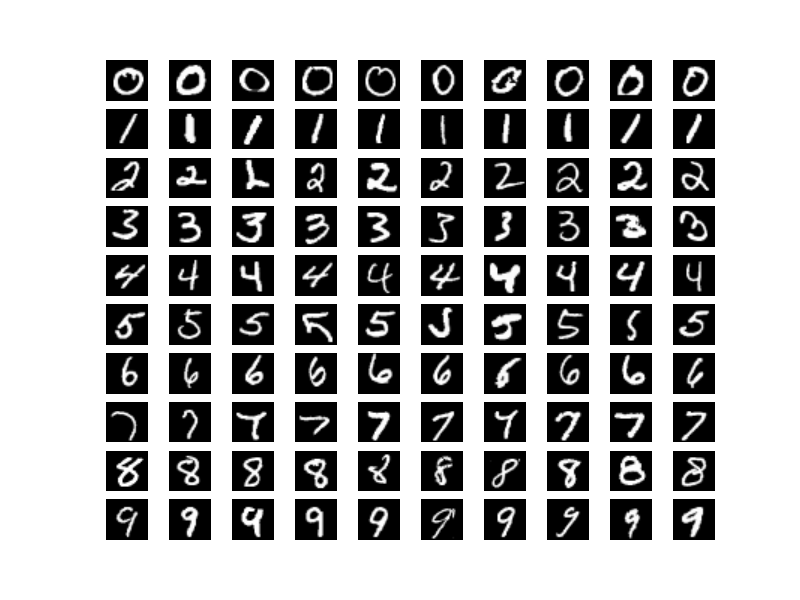
\includegraphics[width=.8\linewidth]{images/1/sample.png}
		\caption{Full data}
		\label{fig:sample}
	\end{figure}

	\begin{figure*}[!ht]
		\begin{subfigure}{.33\textwidth}
			\centering
			
\includegraphics[width=.35\linewidth]{images/1/5_0.png}
			\caption{$5$ but looks like a $3$}
			\label{fig:incorrect1}
		\end{subfigure}
		\begin{subfigure}{.33\textwidth}
			\centering
			
\includegraphics[width=.35\linewidth]{images/1/6_4.png}
			\caption{$6$ but looks like a $4$}
			\label{fig:incorrect2}
		\end{subfigure}
		\begin{subfigure}{.33\textwidth}
			\centering
			
\includegraphics[width=.35\linewidth]{images/1/9_9.png}
			\caption{$9$ but looks like an $8$}
			\label{fig:Incorrect3}
		\end{subfigure}
		\caption{Inaccurate Labels}
		\label{fig:Incorrect}
	\end{figure*}

	\end{homeworkProblem}
	\clearpage

	%---------------------------------------------------------------------------------
	%	PROBLEM 2
	%---------------------------------------------------------------------------------
	\begin{homeworkProblem}
		The output should be:
		\begin{align*}
		o^{(i)} = \sum \limits_{j} w_j x^{(i)}_{j} + b^{(i)}
		\end{align*}
		The listing of the implementation is as follows:\\
		\begin{lstlisting}[language=python, caption=code for linear net output]
	def linear_forward(x, W):
		lin_output = np.dot(W.T, x)
		return softmax(lin_output)
		\end{lstlisting}

	\end{homeworkProblem}
	\clearpage

	%----------------------------------------------------------------------------------
	%	PROBLEM 3
	%---------------------------------------------------------------------------------
	\begin{homeworkProblem}
	
	\begin{enumerate}
		\item 
		Let the loss function $C$ be defined as:
		\begin{align*}
			C &= - \sum \limits_{i} y^{(i)} log ( p_{i} )
		\end{align*}
		
		where $p_{i}$ is:
		\begin{align*}
			p_{i} &= \dfrac{e^{o_i}}{\sum \limits_{j} e^{o_j}}
		\end{align*}
		
		and $o_i$ is:
		\begin{align*}
			o_{i} &= \sum \limits_{j} x^{(i)}_{j} w_{ij} + b_i
		\end{align*}
		
		The gradient for the loss function with respect to the weight $w_{ij}$ $\dfrac{\partial C}{\partial w_{ij}}$ is:
		\begin{align*}
			\dfrac{\partial C}{\partial w_{ij}} = \dfrac{\partial C}{\partial o_{i}} \dfrac{\partial o_{i}}{\partial w_{ij}}
		\end{align*}
		
		Note:
		\begin{align*}
		\dfrac{\partial p_{k}}{\partial o_{i}} &= 
		\begin{cases}
		-p_k p_i       & \textrm{ if } k \neq i \\
		p_i (1 - p_i)  & \textrm{ if } k = i
		\end{cases}
		\end{align*}
		
		Then:
		\begin{align*}
			\dfrac{\partial C}{\partial o_{i}} &= - \dfrac{\partial C}{\partial p_{i}} \dfrac{\partial p_{i}}{\partial o_{i}} + \sum \limits_{k \neq i} \dfrac{\partial C}{\partial p_{k}} \dfrac{\partial p_{k}}{\partial o_{i}} \\
			&= - \dfrac{y^{(i)} }{ p_{i} } p_{i} (1 - p_{i}) + \sum \limits_{k \neq i} \dfrac{y^{(k)}}{p_{k}} p_{k}p_i \\
			&= p_{i} y^{(i)} - y^{(i)} + \sum \limits_{k \neq i} y^{(k)} p_{i} \\
			&= \sum \limits_{k} y^{(k)} p_{i} - y^{(i)} \\
			&= p_{i} - y^{(i)}
		\end{align*}
		
		Also, 
		\begin{align*}
		\dfrac{\partial o_{i}}{\partial w_{ij}} &= x_j^{(i)}
		\end{align*}		
		
		Then
		\begin{align*}
		\dfrac{\partial C}{\partial w_{ij}} &= \dfrac{\partial C}{\partial o_{i}} \dfrac{\partial o_{i}}{\partial w_{ij}} \\
		&= x_{j}^{(i)} (p_{i} - y^{(i)})
		\end{align*}
		
		\newpage
		\item
		The vectorized implementation is as follows:
		\begin{lstlisting}[language=Python, caption=Vectorized gradient]
	def linear_forward(x, W):
		lin_output = np.dot(W.T, x)
		return softmax(lin_output)
	
	def loss(x, W, y):
		p = linear_forward(x, W)
		return -np.sum(y * np.log(p)) / x.shape[1]
	
	def dlossdw(x, W, y):
		p = linear_forward(x, W)
		return np.matmul((p - y), x.T).T
		\end{lstlisting}
		
	\end{enumerate}
	
	
	\end{homeworkProblem}
	\clearpage

	%----------------------------------------------------------------------------------
	%	PROBLEM 4
	%---------------------------------------------------------------------------------
	\begin{homeworkProblem}
		The learning curve is plotted in Fig \ref{fig:4.1}, and the weights going to the output is in Fig \ref{fig:4.2}. The learning curve is as expected: the loss for the training set decreases gradually and the loss for the test set first decreases then increases. The weights' visualization gives each handwritten digits form 0 to 9.
		
		The weights are initialized to $0.5$. This is because if the weights are initialized to 0, the network will not change at all. The learning rate is set to $0.00005$. This is the best value for the network to change and does not overstep the minima
		
		\begin{figure}[!ht]
			\centering
			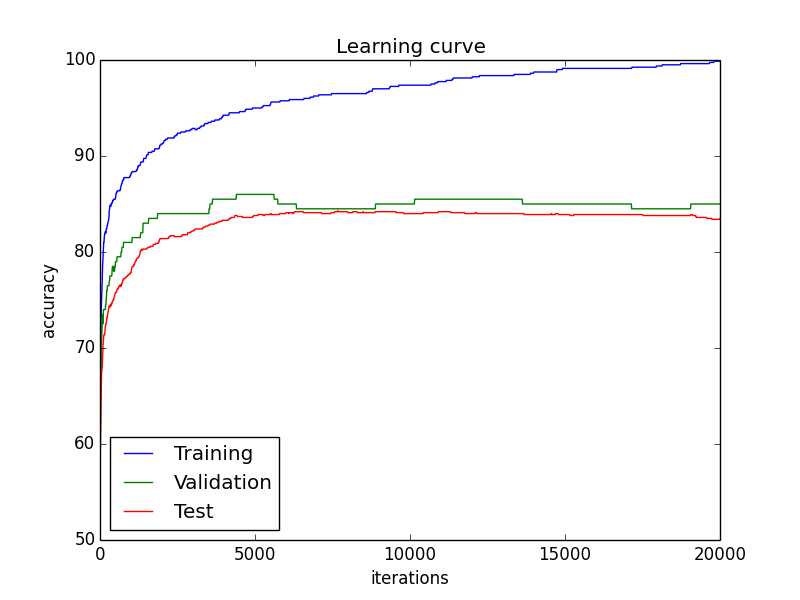
\includegraphics[width=.5\linewidth]{images/4/gradient_descent.png}
			\caption{learning curve}
			\label{fig:4.1}
		\end{figure}
	
		\begin{figure}[!ht]
			\centering
			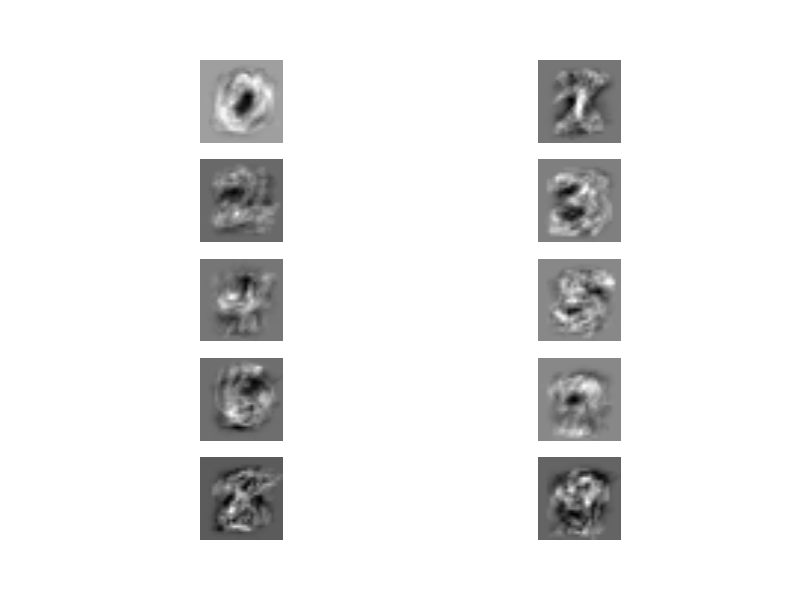
\includegraphics[width=.5\linewidth]{images/4/weights.png}
			\caption{weights}
			\label{fig:4.2}
		\end{figure}


	\end{homeworkProblem}
	\clearpage

	%----------------------------------------------------------------------------------
	%	PROBLEM 5
	%---------------------------------------------------------------------------------
	\begin{homeworkProblem}
		The new code for gradient descent with momentum is as follows:
		\begin{lstlisting}[language=Python, caption= Gradient descent with momentum]
	while i < max_iter and norm(W - prev_W) > eps:
		prev_W = W.copy()
		# W -= alpha * dlossdw(x_train, W, y_train)
		V = gamma * V + alpha * dlossdw(x_train, W, y_train)
		W -= V
		i += 1
		\end{lstlisting}
		
		The learning curve is plotted in Fig \ref{fig:5.1}. Comparing the learning curve to Part 4, the training set learns faster and the test set first decreases and then keeps constant
		
		\begin{figure}[!ht]
			\centering
			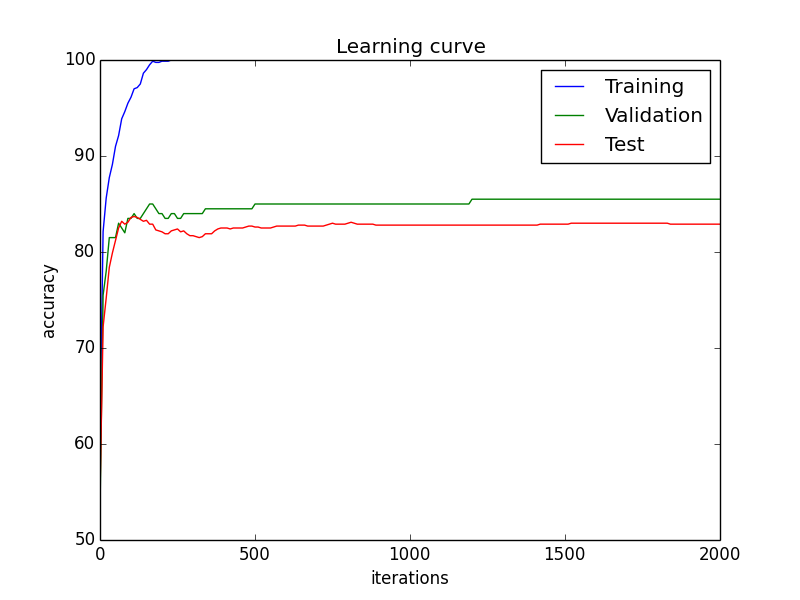
\includegraphics[width=.5\linewidth]{images/5/gradient_descent.png}
			\caption{weights}
			\label{fig:5.1}
		\end{figure}
		
		

	\end{homeworkProblem}
	\clearpage

	%----------------------------------------------------------------------------------
	%	PROBLEM 6
	%---------------------------------------------------------------------------------
	\begin{homeworkProblem}
	
	\begin{enumerate}
		\item 
		The contour plot is given in Fig \ref{fig:6.1}
		
		\item 
		The trajectory for "vanilla" gradient descent is the yellow line in the plot

		\item 
		The trajectory for momentum gradient descent is the green line in the plot

		\item 
		The "vanilla" gradient descent has more fluctuations due to the large learning rate. However, with momentum pointing to the constant optimum direction, the trajectory for momentum has less fluctuations. Also, to achieve the same learning effect (how close to the optimum), momentum gradient descent needs less steps.
		
		\item 
		The points were selected to be around the middle of the image. This is because that is where the weights matter the most. If the points were selected to be at the edge of the image, the weights won't matter because the edge does not contain anything that determines what the digit is.
		
		To produce a good visualization, the learning rate for both gradient descent must be tuned to be higher than normal, and the learning rate for "vanilla" gradient descent must be much higher to produce the fluctuation.
		
		A set of weights that won't produce a good visualization is chosen to be at the corner of the graph. The trajectories are not moving at all no matter how we change the initial values.
		
		\begin{figure}[!ht]
			\centering
			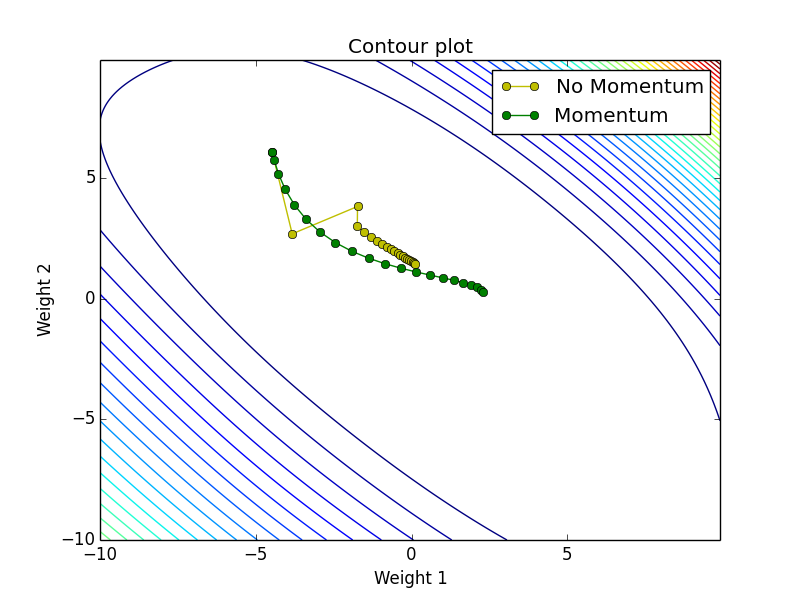
\includegraphics[width=.5\linewidth]{images/6/a.png}
			\caption{part (a-c)}
			\label{fig:6.1}
		\end{figure}
		
	\end{enumerate}

	\end{homeworkProblem}
	\clearpage

	%----------------------------------------------------------------------------------
	%	PROBLEM 7
	%---------------------------------------------------------------------------------
	\begin{homeworkProblem}
		


	\end{homeworkProblem}
	\clearpage

	%----------------------------------------------------------------------------------
	%	PROBLEM 8
	%---------------------------------------------------------------------------------
	\begin{homeworkProblem}
		The final test result for resolution of $32 \times 32$ has an accuracy of $83.3\%$ and for resolution of $64 \times 64$ has an accuracy of $80\%$. The learning curves of the two resolutions are shown in Fig \ref{fig:8.1}.
		
		The results are trained by  a fully connected, three-layered (input, hidden, output) network. The weights and bias are randomized. The activation function for input and output layer is linear, and for the hidden layer is ReLU. The network uses Adam as its optimizer. The hyper-parameters are picked through repeated experiments. The final hyper-parameters are: alpha = 0.001, number of hidden neurons = 36, epoch = 5, number of mini-batch in each epoch = 5, and the number of iterations = 1000
		
		\begin{figure}[!ht]
			\begin{subfigure}{.45\textwidth}
				\centering
				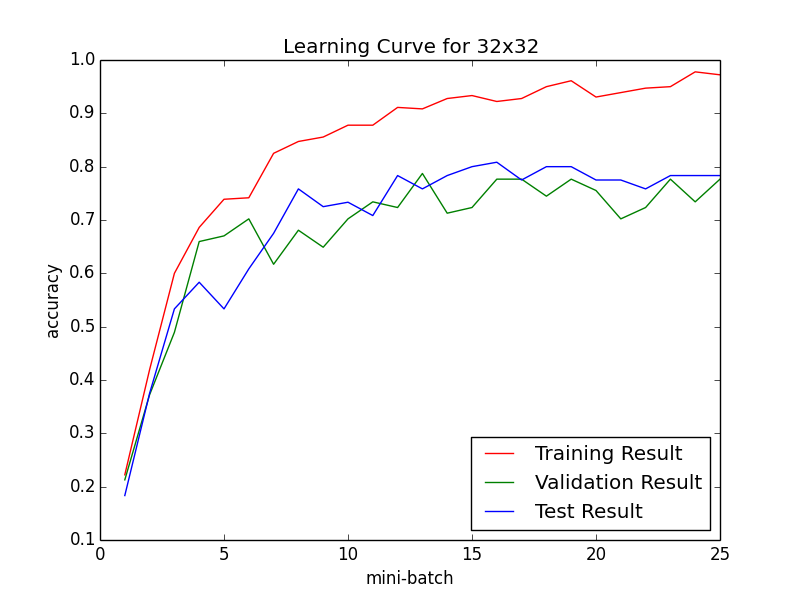
\includegraphics[width=\linewidth]{images/8/a.png}
				\caption{$32 \times 32$}
				\label{fig:8.1a}
			\end{subfigure}
			\begin{subfigure}{.45\textwidth}
				\centering
				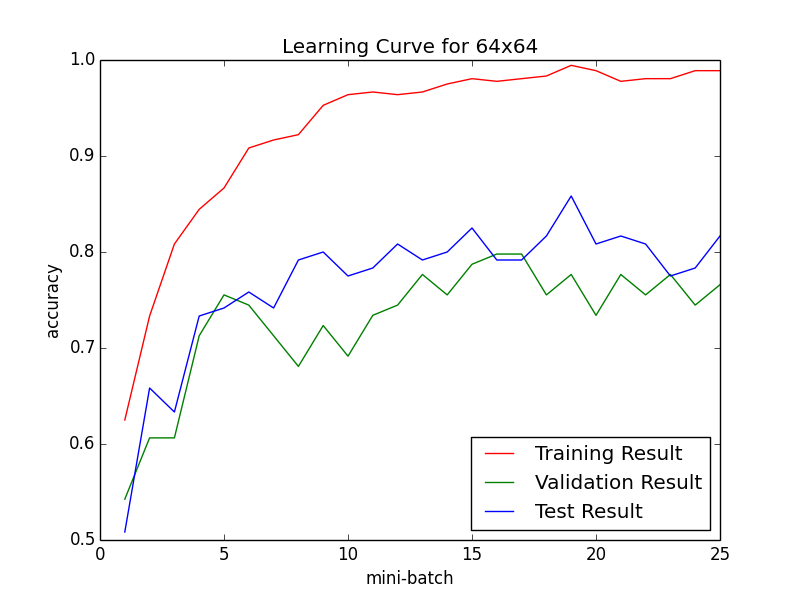
\includegraphics[width=\linewidth]{images/8/b.png}
				\caption{$64 \times 64$}
				\label{fig:8.1b}
			\end{subfigure}
		\centering
		\caption{learning curves}
		\label{fig:8.1}
		\end{figure}


	\end{homeworkProblem}
	\clearpage

	%---------------------------------------------------------------------------------
	%	PROBLEM 9
	%---------------------------------------------------------------------------------
	\begin{homeworkProblem}
		The actors are chosen to be Harmon and Hader. Their hidden units are visualized as in Fig \ref{fig:9}.
		
		The weight units are chosen using the following snippet of code: 
		\begin{lstlisting}[language=Python, caption={Code for choosing featuring weight unit}]
	x = Variable(torch.from_numpy(W), 
		requires_grad=False).type(dtype_float)
	y = model(x).data.numpy()
	for k in range(y.shape[0]):
	print k, actor_names[np.argmax(y[k, :])]
		\end{lstlisting}
		
		\begin{figure}[!ht]
			\begin{subfigure}{.4\textwidth}
				\centering
				
\includegraphics[width=\linewidth]{images/9/0.png}
				\caption{Actor1: Harmon}
				\label{fig:9.1}
			\end{subfigure}
			\begin{subfigure}{.4\textwidth}
				\centering
				
\includegraphics[width=\linewidth]{images/9/2.png}
				\caption{Actor2: Hader}
				\label{fig:9.2}
			\end{subfigure}
			\centering
			\caption{Weight Visualizations}
			\label{fig:9}
		\end{figure}


	\end{homeworkProblem}
	\clearpage

	%----------------------------------------------------------------------------------
	%	PROBLEM 10
	%---------------------------------------------------------------------------------
	\begin{homeworkProblem}
		%		\noindent \textit{Question}


	\end{homeworkProblem}
	\clearpage

	%----------------------------------------------------------------------------------

\end{document}
